
\section{Editor: how to?}
\index{secrets!Editor: how to?}

Here we describe some tips.

\subsection{Macros: how to use?}
\index{secrets!macros}

Tinn-R provides a useful macro option to help you with repetitive actions.


\includegraphics[scale=0.50]{./res/secrets_macro.png}

Click on \texttt{Tools/Macro} at the main menu bar. You will then see two icons: Record \texttt{F7} and Play \texttt{F8}.
Those icons may also be found on the editor task bar. Here is an example: write a vector 1:20 and send it to \RR{}.
In the Rterm window you will then see the numbers 1 to 20 in a single line. Copy and paste that to the editor's window.

Suppose that you want to write a comma after every number, maintaining a one space distance after the comma.
Place the cursor just before the number one and then press \texttt{F7}.
A \texttt{+} sign will appear on the Record icon at the editor taskbar, meaning that you are beginning to record action
you take on the screen. Press the right arrow to move across the number 1 and type a comma (,),
delete one space and move the cursor one space to the right with the right arrow and press again
\texttt{F7} to stop the recording process. The little \texttt{+} sign will disappear.
Now just press \texttt{F8} and see what happens. When you reach the number ten it won't work because now the numbers
consists of two digits and the spacings will not fit.
After doing that for the number nine the cursor will stop in the middle of the number ten,
go back one step to the left with the left arrow, and press space bar so that there will be one blank space
between the comma and the number ten. Now press again \texttt{F7} go across the number ten with the right arrow
type the comma (,) and go one space to the right with the right arrow so the cursor is now at the left side of
the number eleven, press again \texttt{F7}, and then \texttt{F8} until the end.
Try now to write those numbers in a vertical line across the left margin without the commas using again the macros.

\subsection{Marks: how to use?}
\index{secrets!marks}

One very useful navegation tool is the \texttt{bookmark}. To define the bookmark,
use \texttt{CTRL + SHIFT + [0-9]} (a key from 0 to 9) on the line you chose.
Then, to go to the corresponding bookmark just use \texttt{CTRL + [0-9]}.
A visual indicator appears in the left margin, just before the line number, of that line.
Suppose you are working on a long script and need to constantly return to a specified line.
You will see how handy it is. To undo it, just use again \texttt{CTRL + SHIFT + [0-9]} using the same number, on the same line.

You may also mark a whole block. To to that, first select the block and then click on Marks at the main menu and click on mark.
As in the above paragraph the number 0 will appear at the begining of the block and the number 1 at the end.
You can modify the box and send it to \RR{} to be processed.

\subsection{Editor, Tools and Rterm: how to arrange?}
\index{secrets!arrange}

\texttt{CTRL + F8} toggles the visibility of window \texttt{Tools} and \texttt{CTRL + F9}
toggles the visibility of window \texttt{Rterm}. Now press \texttt{CTRL + F10},
\texttt{CTRL + F11} or \texttt{CTRL + F12} and see what happens.

The use of two monitors is recommended in case of intensive use.
Placing \RR{} (Rgui or Rterm) on a second monitor makes working with data analysis and development tasks very comfortable.

\subsection{Active page using the keyboard: how to change?}
\index{secrets!active page}

\begin{verbatim}
CTRL + TAB         : Change sequentially the active page to the right
                     (requires more than one)
CTRL + SHIFT + TAB : Change sequentially the active page to the left
                     (requires more than one)
\end{verbatim}

\subsection{Tab order: how to change?}
\index{secrets!tab order}

Drag and drop the tab to the left or right.

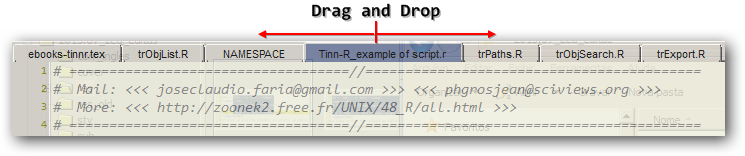
\includegraphics[scale=0.50]{./res/filetabs.png}
